\chapter{Revisão Bibliográfica}
%% Visão geral sobre carregadores de veículos elétricos.

O artigo de \cite{Yuan:2021} faz uma revisão sistemática sobre carregadores \textit{onboard}
bidirecionais e aborda sobre os principais modelos comerciais presentes no mercado. Dentre os
sistemas de carregamento trifásico citados há o carregador trifásico da \textit{Current Ways}
que oferece uma potência de saída de até 26,4 kW, uma tensão de saída na faixa de 250 V a 425 V
e eficiência em torno de 96 \%. A estrutura interna do carregador é composta por retificador
PFC ativo de ponte completa e um conversor CC-CC isolado DAB. Já o carregador da \textit{EATON}
fornece uma potência de saída de até 22 kW com uma tensão de saída na faixa de 225 V a 500 V e
eficiência de 95 \%. A empresa não detalha sobre a composição interna do carregador.

O texto de \cite{Yuan:2021} também revisa as principais tecnologias que são utilizadas
atualmente nos carregadores.

\cite{Baharom:2024} comentam sobre futuros avanços tecnológicos no carregamento de veículos elétricos. O texto aborda especificamente sobre os desafios de desenvolver um carregador onboard bidirecional, que incluem a dificuldade de gerenciar o fluxo de potência em ambos os sentidos, a complexidade necessária para o sistema de controle e a integração desses sistemas com a rede elétrica existente. Ademais, o artigo aborda sobre o carregamento indutivo sem fio e justifica a necessidade em pesquisa nessa tecnologia com base na maior segurança e menor necessidade de manutenção obtida. Ao mesmo tempo, os autores reconhecem que a limitação na transferência de potência sem fios e a baixa eficiência inviabilizam esse sistema na prática.

De acordo com \cite{Kumar:2021}, os convesores CA-CC bidirecionais, que estão presentes em
carregadores de carros elétricos, apresentam desafios em relação a sincronização de frequência
e fase, controle do fator de potência e qualidade de isolação.

%% Visão sobre o PFC.

Os \textit{application notes} \cite{onsemi_hbd853} e \cite{ti_zhcp224} apresentam uma visão
geral sobre o controle do fator de potência ativo com um conversor boost monofásico. Esse
conversor pode operar tanto em modo de condução contínua (CCM) quanto em modo de condução
crítica (CRM). Em CCM, o conversor é controlado através do controle pelo modo de corrente
média. Nesse cenário, a malha de controle externa é lenta e tem o papel de ajustar o valor de
tensão de saída enquanto que a malha de controle de corrente(interna) é mais rápida e visa
fazer com que a corrente média do indutor siga a forma de onda de uma entrada de referência
senoidal que esteja em fase com a tensão da rede. Já a operação em CRM é adequada apenas para
uma potência de saída abaixo de 300 W e caracteriza-se pelo controle através de um sinal PWM
com frequência de cheaveamento variável e tempo ON constante.

O artigo da ONSEMI \cite{onsemi_h2ptoday2102} aborda as principais topologias de retificadores
PFC trifásicos. A primeira topologia citada é o retificador PWM Vienna (Fig.
\ref{fig:pfc_vienna}), que é caracterizada como uma ponte retificadora trifásica conectada a
uma conversor boost por fase. A topologia Vienna tem como principal vantagem o uso de apenas um
transistor por fase, o que simplica significativamente o controle do conversor e o cheaveamento
em três níveis, ao mesmo tempo, o alto número de diodos nessa topologia implica em maiores
perdas. Já topologia T-NPC (Fig. \ref{fig:pfc_tnpc}) é derivada da Vienna e consiste
basicamente numa ponte de diodos trifásica conectada a seis transistores. A principal vantagem
dessa topologia é o menor número de componentes em relação à anterior. Ambas as topologias
citadas são unidirecionais. Ademais, a topologia T-NPC pode ser implementada apenas com
transistores, o que a torna bidirecional.

\begin{figure}[h]
	\centering
	\begin{minipage}{0.45\textwidth}
		\centering
		\caption{Retificador PFC Vienna.}
		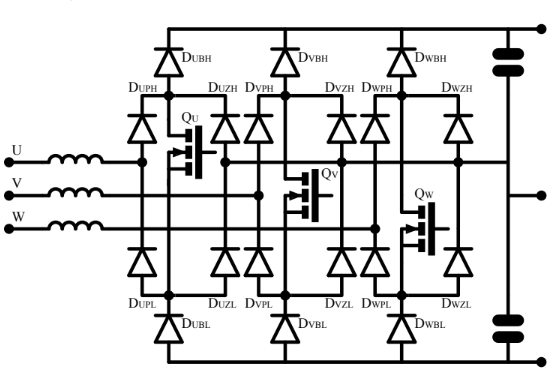
\includegraphics[width=\textwidth]{./Figuras/PFC_Vienna.png}
		\legend{Fonte: \cite{onsemi_h2ptoday2102}}
		\label{fig:pfc_vienna}
	\end{minipage}
	\hfill
	\begin{minipage}{0.45\textwidth}
		\centering
		\caption{Retificador T-NPC.}
		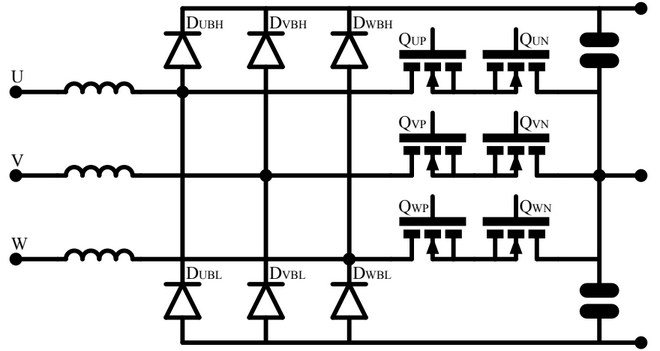
\includegraphics[width=\textwidth]{./Figuras/PFC_TNPC.png}
		\legend{Fonte: \cite{onsemi_h2ptoday2102}}
		\label{fig:pfc_tnpc}
	\end{minipage}
\end{figure}

A principal topologia de retificador PFC trifásico é o \textit{Six-switch rectifier} vista na
Figura \ref{fig:pfc_six_switch}, que consiste numa ponte trifásica formada por seis
transistores de tensão nominal na faixa de 900 V a 1200 V. A principal vantagem dessa topologia
é a bidirecionalidade, inclusive porque o inversor trifásico a seis transistores é
frequentemente utilizado no acionamento de motores elétricos \cite{onsemi_h2ptoday2102}. Ao
mesmo tempo, esse retificador apresenta maior interferência eletromagnética que as outras
opções citadas e opera com chaveamento em dois níveis.

\begin{figure}
	\centering
	\caption{Retificador trifásico PFC de ponte completa.}
	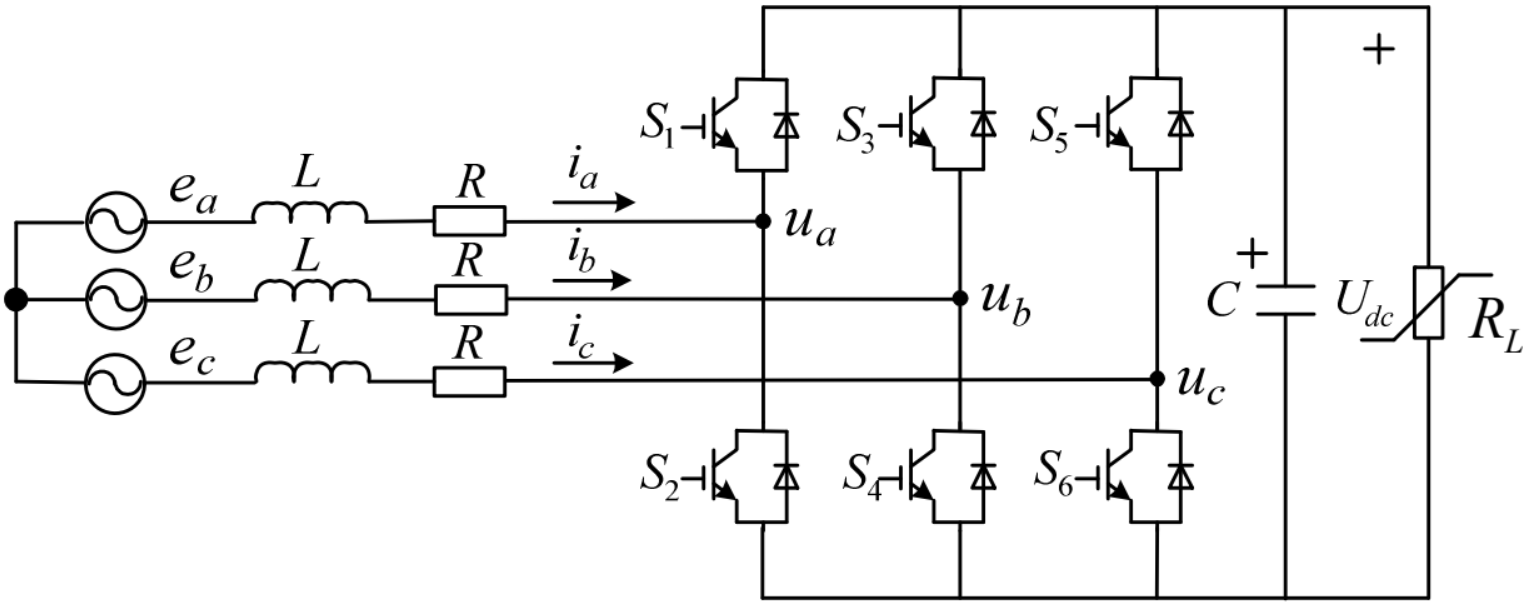
\includegraphics[width=0.7\textwidth]{./Figuras/retificador_six_switch.png}
	\legend{Fonte: \cite{WANG2013/03}}
	\label{fig:pfc_six_switch}
\end{figure}

%% Controle do PFC Trifásico

Em relação ao retificador PFC trifásico, tanto \cite{3phPlecs} quanto \cite{WANG2013/03}
realizam o controle do conversor CA-CC por meio da transformada de Park. Nessa metodologia, um
\textit{Phase Locked Loop} (PLL) captura a referência de fase da tensão de entrada, que em
seguida é utilizada na transformação para o sistema de coordenadas dq0.Ademais, duas malhas de
controle, uma externa, referente à tensão de saída do retificador e uma interna, que controla
as componentes de eixo direto e em quadratura da corrente de entrada. Como o objetivo é
controlar o fator de potência, a componente de corrente em quadratura é ajustada para ser nula.

A nota de aula \cite{dq0_transform} explica sobre como aplicar a Transformada de Park em um
modelo de circuito trifásico modelado em espaços de estados. Já o livro \cite{} aborda sobre os
quadros de referência \(\alpha \beta\) e dq0, utilizados na Transformada de Clarke e na
Transformada de Park, respectivamente.

%% Conversor CC-CC isolado

O \textit{application note} da Infineon \cite{Infineon_CoolMOS_CFD7A} aborda sobre as
principais topologias de conversores CC-CC isolados utilizados nos carregadores
\textit{onboard} de veículos elétricos. O \textit{Phase Shifted Full Bridge} é composto por uma
ponte completa ativa, um transformador e uma ponte retificadora e caracteriza-se pela alta
eficiência, uso de comutação suave e controle do fluxo de potência pelo ajuste da desafasagem
de tensão entre os dois braços da ponte de transistores. O \textit{Dual Active Bridge}
substitui os diodos da ponte retificadora por transistores, permitindo a bidirecionalidade.
Para garantir maior eficiência, o conversor ressonante LLC é utilizado por conta da capacidade
de operar com \textit{Zero Voltage Switching}(ZVS). Ao mesmo tempo, os conversores ressonantes
apresentam maior complexidade, pois são controlados com frequência variável ao invés de uma
razão cíclica variável.

